\documentclass[12pt,letterpaper]{book}
\usepackage[utf8]{inputenc}
\usepackage[spanish,es-tabla]{babel}
\decimalpoint
\let\cleardoublepage\clearpage
\usepackage{amsmath}
\usepackage{amsfonts}
\usepackage{amssymb}
\usepackage{esint}
\usepackage{color}
\usepackage{graphicx}
\usepackage{anysize}
\usepackage{anyfontsize}
\usepackage{pdfpages}
\usepackage{makeidx}
\makeindex 
\usepackage{epstopdf}
\usepackage[x11names,table]{xcolor}
\usepackage{tikz}
\usepackage{tcolorbox}
\usepackage[hidelinks]{hyperref}
\usepackage[labelfont=bf]{caption}
\captionsetup[table]{labelsep=space}
\captionsetup[figure]{labelsep=space}
\usepackage{listings}
\usepackage{bm}
% Margenes
\usepackage[left=3cm,top=2.5cm,right=2.5cm,bottom=2.5cm]{geometry}

\setlength{\parindent}{0cm}
\tcbset{colback=green!5!white, colframe=gray!10!black, coltitle=green!20!black, 
fonttitle=\bfseries, colbacktitle=white, coltext=gray!30!black}
\addto\captionsspanish{
    \renewcommand{\figurename}{{\bf Figura}}% 
}
\usepackage{epigraph}
\usepackage{xcolor}
\usepackage{textcomp}
\usepackage{gensymb}

% \renewcommand{\familydefault}{\sfdefault}

% Colores
\definecolor{verdep}{rgb}{0.5,0.5,0.9}
\definecolor{ccap}{rgb}{0.2,0.2,0.2}
\definecolor{csec}{rgb}{0.4,0.4,0.4}
\definecolor{csubsec}{rgb}{0.6,0.6,0.6}
\definecolor{cenun}{rgb}{0.2,0.2,0.3}
\definecolor{csol}{rgb}{0.2,0.8,0.1}
\definecolor{backcode}{rgb}{0.98,0.97,0.98}
\definecolor{framecode}{rgb}{0.7,0.7,0.7}
\definecolor{dkgreen}{rgb}{0,0.6,0}
\definecolor{gray}{rgb}{0.5,0.5,0.5}
\definecolor{mauve}{rgb}{0.58,0,0.82}

\definecolor{title_color}{rgb}{0.0, 0.3, 0.0}


\newtcbox{\mybox}[1][red]{on line,
arc=7pt,colback=#1!10!white,colframe=#1!50!black,
before upper={\rule[-3pt]{0pt}{10pt}},boxrule=1pt,
boxsep=0pt,left=6pt,right=6pt,top=2pt,bottom=2pt}


% Nuevos comandos

\renewcommand{\vec}[1]{\mathbf{#1}}

\usepackage{titlesec}%--
\newcommand{\hsp}{\hspace{5pt}}
%\titleformat{\chapter}[hang]{\huge\bfseries\color{ccap}}
%{\color{verdep}{\vrule height 2.5cm width 1mm}\hsp{\fontsize{100}{5}\selectfont\thechapter}\hsp%
%{\vrule height 2.5cm width 1mm}\hsp{\fontsize{30}{5}\selectfont}}{5pt}{\huge\bfseries}

% \titleformat{\chapter}[hang]{\huge\bfseries\color{ccap}}
% {\color{verdep}\hsp{\fontsize{30}{5}\selectfont Capítulo \thechapter.\\}\hsp%
% \hsp{\fontsize{30}{5}\selectfont}}{5pt}{\huge\bfseries}

% \titleformat{\section}[hang]{\normalfont\color{csec}}%
% {\filright\large\enspace\thesection\enspace}%
% {8pt}{\Large\bfseries\filright}%

% \titleformat{\subsection}[hang]{\normalfont\color{csec}}%
% {\filright\large\enspace\thesubsection\enspace}%
% {8pt}{\large\bfseries\filright}%

% Code

\lstnewenvironment{python}{\lstset{frame=single,
    frameround=tttt,
    backgroundcolor=\color{backcode},
    rulecolor = \color{framecode},
    language=python,
    aboveskip=3mm,
    belowskip=3mm,
    showstringspaces=false,
    columns=flexible,
    basicstyle={\small\ttfamily},
    numbers=none,
    numberstyle=\tiny\color{gray},
    keywordstyle=\color{blue},
    commentstyle=\color{dkgreen},
    stringstyle=\color{mauve},
    breaklines=true,
    breakatwhitespace=true,
    tabsize=3,
    extendedchars=true,
    inputencoding=utf8,
    literate=%
    {°}{{\,\,$^\circ$\,\,}}1
    {á}{{\'a}}1
    {é}{{\'e}}1
    {í}{{\'i}}1
    {ó}{{\'o}}1
    {ú}{{\'u}}1
    {Á}{{\'A}}1
    {É}{{\'E}}1
    {Í}{{\'I}}1
    {Ó}{{\'O}}1
    {Ú}{{\'U}}1
}}{}

\author{\textit{P.J. De Los Santos}}

\title{
{\bfseries\color{title_color} NuSA, análisis numérico estructural utilizando Python} \\
}


% ======================================================================================================
\begin{document}
\maketitle

\frontmatter
\tableofcontents

% ==================================================== Contenido ====================================================
\mainmatter
% \makeatletter
\def\thickhrulefill{\leavevmode \leaders \hrule height 1ex \hfill \kern \z@}
\def\@makechapterhead#1{%
  \reset@font
  \parindent \z@ 
  \vspace*{15\p@}%
  \hbox{%
    \vbox{\hsize=2cm
      \begin{tabular}{c}
        \scshape \strut \@chapapp{} \\
        \fbox{%
          \vrule depth 10em width 0pt%
          \vrule height 0pt depth 0pt width 2ex%
          {\Huge  \bfseries \strut  \thechapter}%
          \vrule height 0pt depth 0pt width 2ex%
          }
      \end{tabular}%
      }%
    \vbox{%
      \advance\hsize by -2cm
      \hrule\par
      \vskip 6pt%
      \hspace{1em}%
      \LARGE \bfseries #1
      }%
    }%
  \vskip 100\p@
}
\def\@makeschapterhead#1{%
  \reset@font
  \parindent \z@ 
  \vspace*{10\p@}%
 \hbox{%
    \vbox{\hsize=3cm
      \begin{tabular}{c}
        \scshape \strut \vphantom{\@chapapp{}} \hphantom{\@chapapp{}} \\
        \fbox{%
          \vrule depth 5em width 0pt%
          \vrule height 0pt depth 0pt width 1ex%
          {\LARGE \bfseries \strut \hphantom{\thechapter}}%
          \vrule height 10pt depth 0pt width 1ex%
          }
      \end{tabular}%
      }%
    \vbox{%
      \advance\hsize by -2cm    
      \hrule\par
      \vskip 8pt%
      \hspace{1em}%
      \LARGE \bfseries #1
      }%
    }%
  \vskip 100\p@
}
 % Setting for chapters
\chapter{Una introducción a NuSA}

\section{¿Qué es NuSA?}

\textbf{NuSA} es una librería Python para resolver problemas de análisis estructural bidimensional. 
La idea es tener una estructura de códigos escritos utilizando la programación orientada a 
objetos, de modo que sea posible crear instancias de un modelo de elemento finito y operar 
con éste mediante métodos de clase.\\

La estructura de \textbf{NuSA} está basada en tres clases fundamentales que componen el \textit{core}: 
\texttt{Model}, \texttt{Node} y \texttt{Element}.

\begin{center}
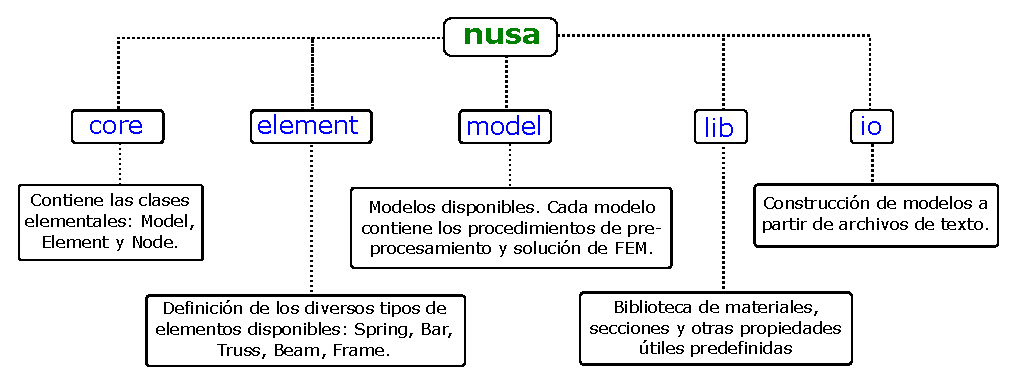
\includegraphics[scale=0.8]{src/intro-nusa/nusa_structure.eps}
\end{center}


\begin{python}
class Model(object):
    """
    Superclass for all FEA models
    """
    def __init__(self,name,mtype):
        self.mtype = mtype # Model type
        self.name = name # Name 
        self.nodes = {} # Dictionary for nodes {number: NodeObject}
        self.elements = {} # Dictionary for elements {number: ElementObject}
        
    def addNode(self,node):
        """
        Add element to current model
        
        *node* :   :class:`~nusa.core.Node`
        """
        current_label = self.getNumberOfNodes()
        if node.label is "":
            node.setLabel(current_label)
        self.nodes[node.label] = node
        
    def addElement(self,element):
        """
        Add element to current model
        
        *element* :  :class:`~nusa.core.Element`
            Element instance 
        
        ::
        
            m1 = Model()
            e1 = Bar(Node((0,0),0),Node((1,0),0))
            m1.addElement(e1)
        
        """
        if self.mtype != element.etype:
            raise ValueError("Element type must be "+self.mtype)
        current_label = self.getNumberOfElements()
        if element.label is "":
            element.setLabel(current_label)
        self.elements[element.label] = element

    def getNumberOfNodes(self):
        return len(self.nodes)
        
    def getNumberOfElements(self):
        return len(self.elements)
        
    def getNodes(self):
        return self.nodes.values()
        
    def getElements(self):
        return self.elements.values()
    
    def __str__(self):
        custom_str = ("Model: "+self.name+"\nNodes: "+str(self.getNumberOfNodes())+
        "\nElements: "+str(self.getNumberOfElements()))
        return custom_str
\end{python}
\chapter{Elemento Spring}

\section{Fundamento teórico}

El elemento \textit{Spring} (resorte) es un elemento finito unidimensional donde 
las coordenadas locales y globales coinciden. Cada elemento spring tiene dos 
nodos como se muestra en la figura \ref{fig:spring_element}. Sea la rigidez del 
resorte la denotada por $k$, en este caso la matriz de rigidez del elemento está 
dada por:

\begin{equation}
K_{(e)} = \begin{bmatrix}
k & -k \\
-k & k 
\end{bmatrix}
\end{equation}

\begin{center}
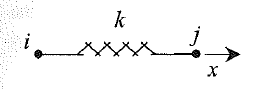
\includegraphics[scale=0.8]{src/spring-element/spring_element.png}
\captionof{figure}{Elemento spring}
\label{fig:spring_element}
\end{center}

Obviamente la matriz de rigidez para un elemento \textit{spring} es de $2\,x\,2$, dado que 
este tiene dos grados de libertada, uno en cada nodo. Consecuentemente para un 
sistema de elementos \textit{spring} con $n$ nodos, el tamaño de la matriz global de 
rigidez $K$ será de $n\,x\,n$. La matriz global de rigidez se obtiene ensamblando 
los matrices de rigidez por elemento $K_{(i)}$ para $i=1,2,...,n$, utilizando el método 
directo de la rigidez.\\

Una vez que la matriz global de rigidez $K$ es obtenida  se tiene un sistema de ecuaciones 
de la forma:

\begin{equation}
[K]\{U\} = \{F\}
\end{equation}

Donde $U$ es el vector global de desplazamientos nodales y $F$ es el vector global de 
fuerzas nodales.\\

El sistema de ecuaciones resultantes se puede simplificar aplicando las condiciones 
de frontera o restricciones de desplazamiento, quedando generalmente un sistema 
de menor dimensión el cuál está determinado y puede resolverse utilizando métodos 
de álgebra lineal´, quedando una posible solución como:

\begin{equation}
\overline{U} = \overline{K}^{-1}\, \overline{F}
\end{equation}

Donde $\overline{U}, \overline{K} \,\, y \,\, \overline{F}$ corresponden a las variables descritas 
anteriormente, después de aplicar las condiciones de frontera correspondientes.


\section{Un ejemplo resuelto en NuSA}

En lo subsecuente se propone un ejercicio de elementos \textit{spring} y se resuelve 
utilizando la librería NuSA.

\textbf{Ejemplo 1.} Para el ensamble mostrado en la figura \ref{fig:example_01}, calcular 
a) la matriz global de rigidez  b) los desplazamientos de los nodos 3 y 4  c) las fuerzas 
de reacción en los nodos 1 y 2, y  d) las fuerzas en cada elemento. Una fuerza de 5000 lb 
es aplicada en el nodo 4 en la dirección $x$, las constantes de rigidez para cada resorte 
se muestran en la figura. Los nodos 1 y 2 están fijos.

\begin{center}
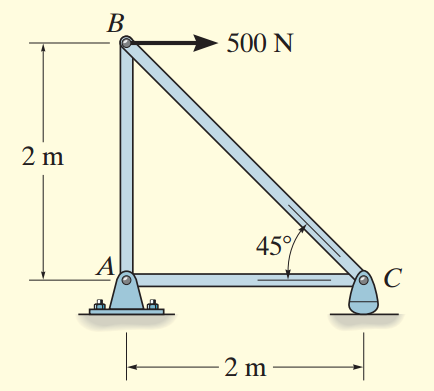
\includegraphics[scale=0.8]{src/spring-element/example_01.png}
\captionof{figure}{}
\label{fig:example_01}
\end{center}



% ==================================================== Referencias ====================================================
\bibliographystyle{unsrt}
\bibliography{references}

\end{document}

% chrome://settings/resetProfileSettings